% !TEX program = xelatex
% A0 縦ポスター — JSIAM 2026（再構成版：1-2紹介 / 3統合 / 4結果 / 今後・参考文献拡大）
\documentclass[25pt, a0paper, portrait,
               margin=15mm, innermargin=8mm,
               blockverticalspace=5mm, colspace=8mm]{tikzposter}

\usepackage{amsmath, amssymb}
\usepackage{graphicx}
\usepackage{booktabs}
\usepackage{xcolor}
\usepackage{qrcode}
\usepackage{xeCJK}
\setCJKmainfont{Noto Serif CJK JP}
\setCJKsansfont{Noto Sans CJK JP}

\definecolor{accent}{HTML}{1F5FE0}
\definecolor{softblue}{HTML}{E6EFFF}
\definecolor{muted}{HTML}{6B7280}
\definecolor{warn}{HTML}{B5322E}

\usetheme{Simple}
\colorlet{backgroundcolor}{white}
\colorlet{blocktitlebgcolor}{softblue}
\colorlet{blocktitlefgcolor}{black}
\colorlet{titlebgcolor}{white}
\colorlet{titlefgcolor}{black}
\usebackgroundstyle{Plain}
\usetitlestyle{Filled}

\newcommand{\ediv}{e_{\mathrm{div}}}
\newcommand{\nunb}{n_{\mathrm{unb}}}
\newcommand{\bt}[1]{{\color{accent}\textbf{#1}}\ }

\tikzposterlatexaffectionproofoff

\title{金融市場の相関ネットワークの位相解析}
\author{赤塩 甫\quad 東京都市大学 賈研究室\quad{\normalsize 指導：賈 伊陽}}
\institute{}

\begin{document}
\maketitle

\begin{columns}

% ================= 左列 =================
\column{0.333}

\block{\bt{1.}動機と問い}{%
株価そのものを\textbf{予測}するのではなく、
危険な局面で株を避けて\textbf{\color{accent}下落を回避}できないか。
そのために、市場の``つながりの形''から\textbf{2つの指標}を作る。

\vspace{2mm}
\textbf{本研究の問い}:
\begin{itemize}
\setlength{\itemsep}{1.5mm}
\item この\textbf{2つの指標は、たがいに独立}か？
\item その2つを\textbf{組み合わせると、下落を回避}できるか？
\end{itemize}

\vspace{2mm}
{\color{muted}\small
\textbf{用語}: \textbf{日次リターン}＝1日の値動き（前日比の変化率）。
\textbf{相関}＝2銘柄の値動きの似方（$+1$＝完全に同調、$0$＝無関係、$-1$＝完全に逆）。}
}

\block{\bt{2.}相関ネットワーク}{%
40銘柄を\textbf{点}、値動きが\textbf{類似した}銘柄どうしを\textbf{線}で結ぶ。
相関 $r$ を距離 $d=\sqrt{2(1-r)}$ に変換し、類似した銘柄を近くに配置する。

\vspace{2mm}
\centering
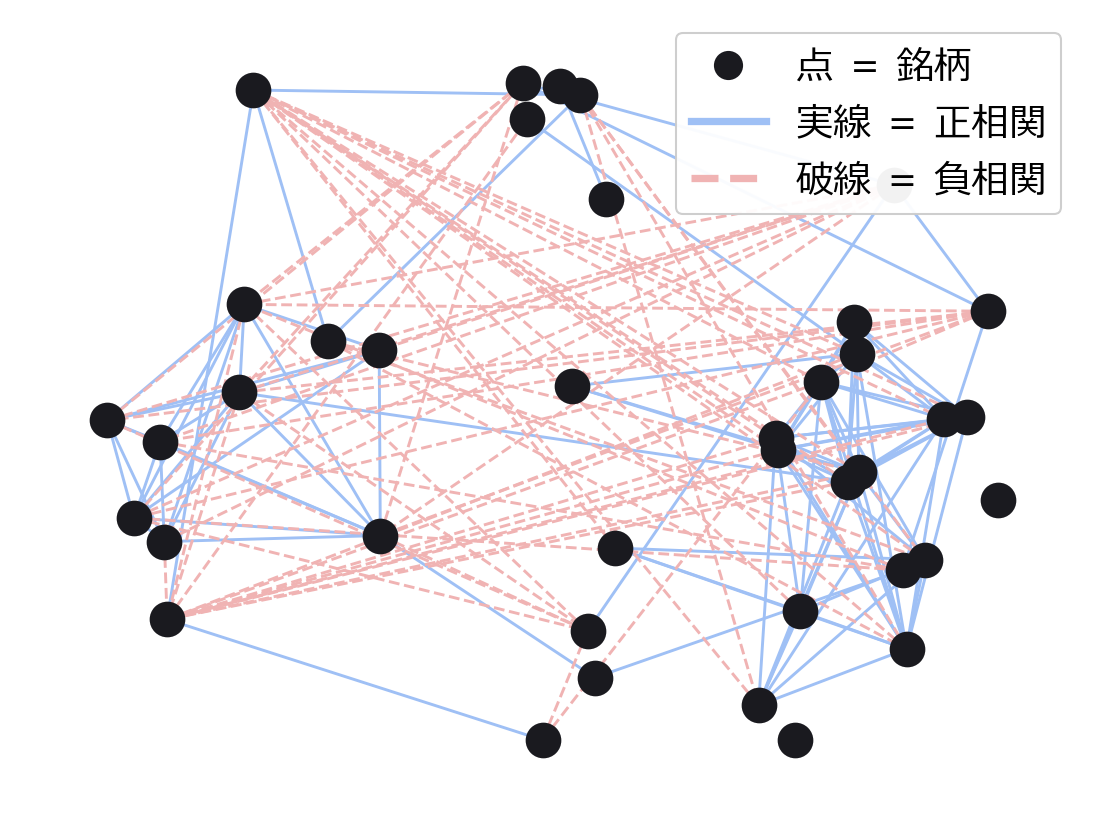
\includegraphics[width=0.72\linewidth]{../../figs/slide_network.png}\\
{\color{muted}\footnotesize 青＝正の相関・赤破線＝負の相関（40銘柄の相関ネットワーク）}

\vspace{2mm}
\raggedright
このネットワークの``形''と``符号''から、次の2つの指標を取り出す（3.1・3.2）。
}

\block{\bt{3.1}指標1：穴の持続期間}{%
ネットワーク上の点を、近いものから順に結んでいく。
その基準を上げると、\textbf{``輪（穴）''が現れ、やがて埋まって消える}。

\vspace{2mm}
\centering
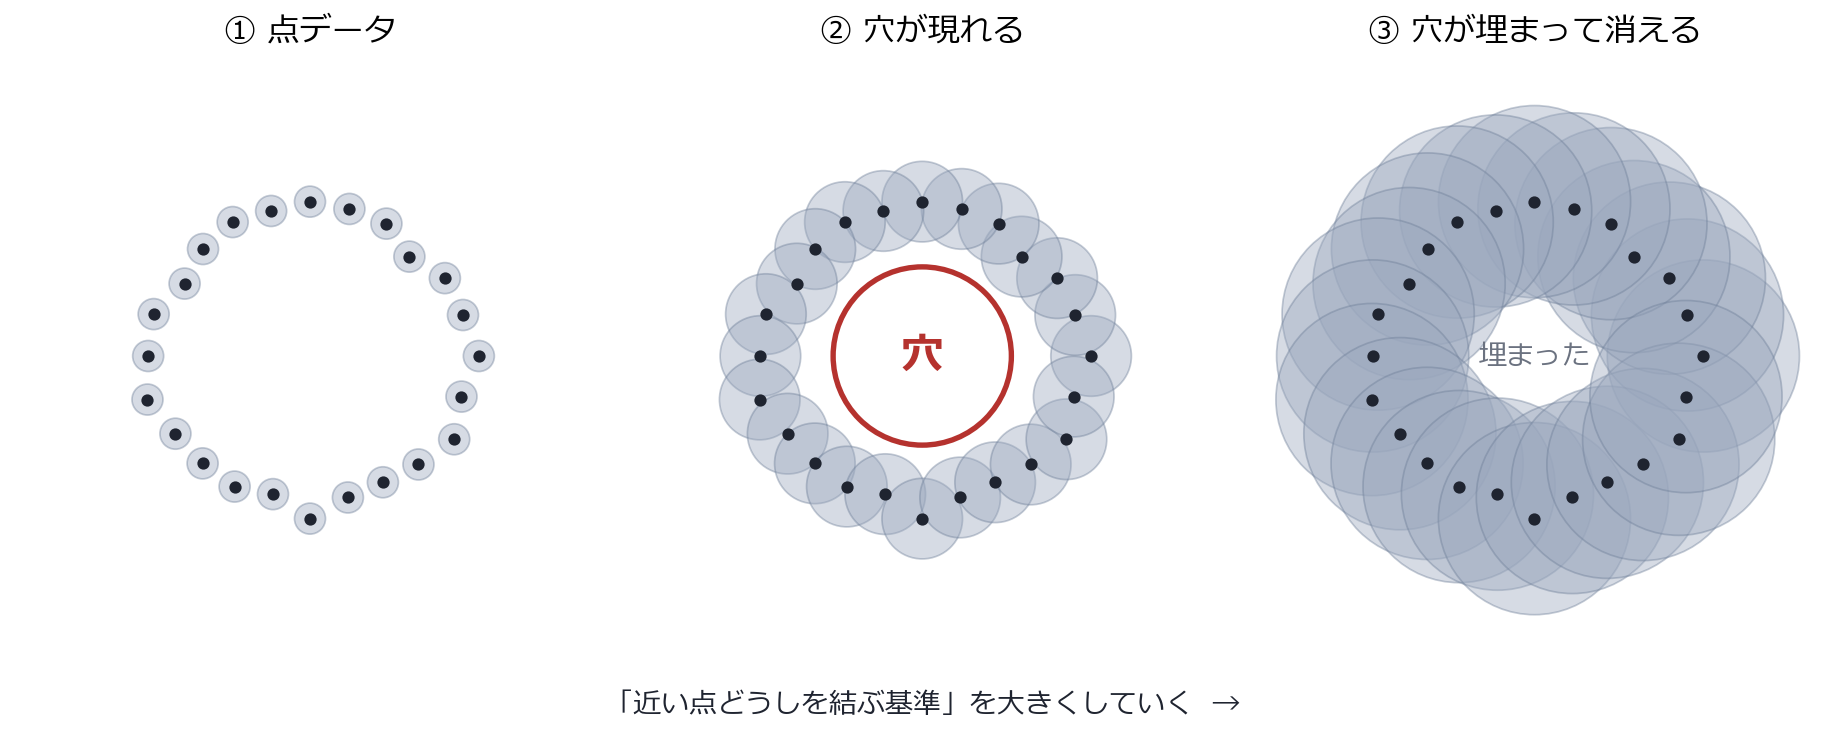
\includegraphics[width=\linewidth]{../../figs/slide_hole.png}

\vspace{1mm}
\raggedright
\begin{itemize}
\setlength{\itemsep}{1mm}
\item \textbf{\color{accent}長く残る穴＝本物の構造}（市場のまとまり）
\item すぐ消える穴＝ノイズ
\end{itemize}
指標 $L^1$ ＝ すべての穴の\textbf{持続期間（消える基準 $-$ 現れる基準）の合計}。
}

% ================= 中列 =================
\column{0.333}

\block{\bt{3.2}指標2：矛盾の数}{%
各線に\textbf{符号}を付ける（正の相関＝$+$、負の相関＝$-$）。
輪を一周して\textbf{符号をかけ合わせる}。

\vspace{2mm}
\centering
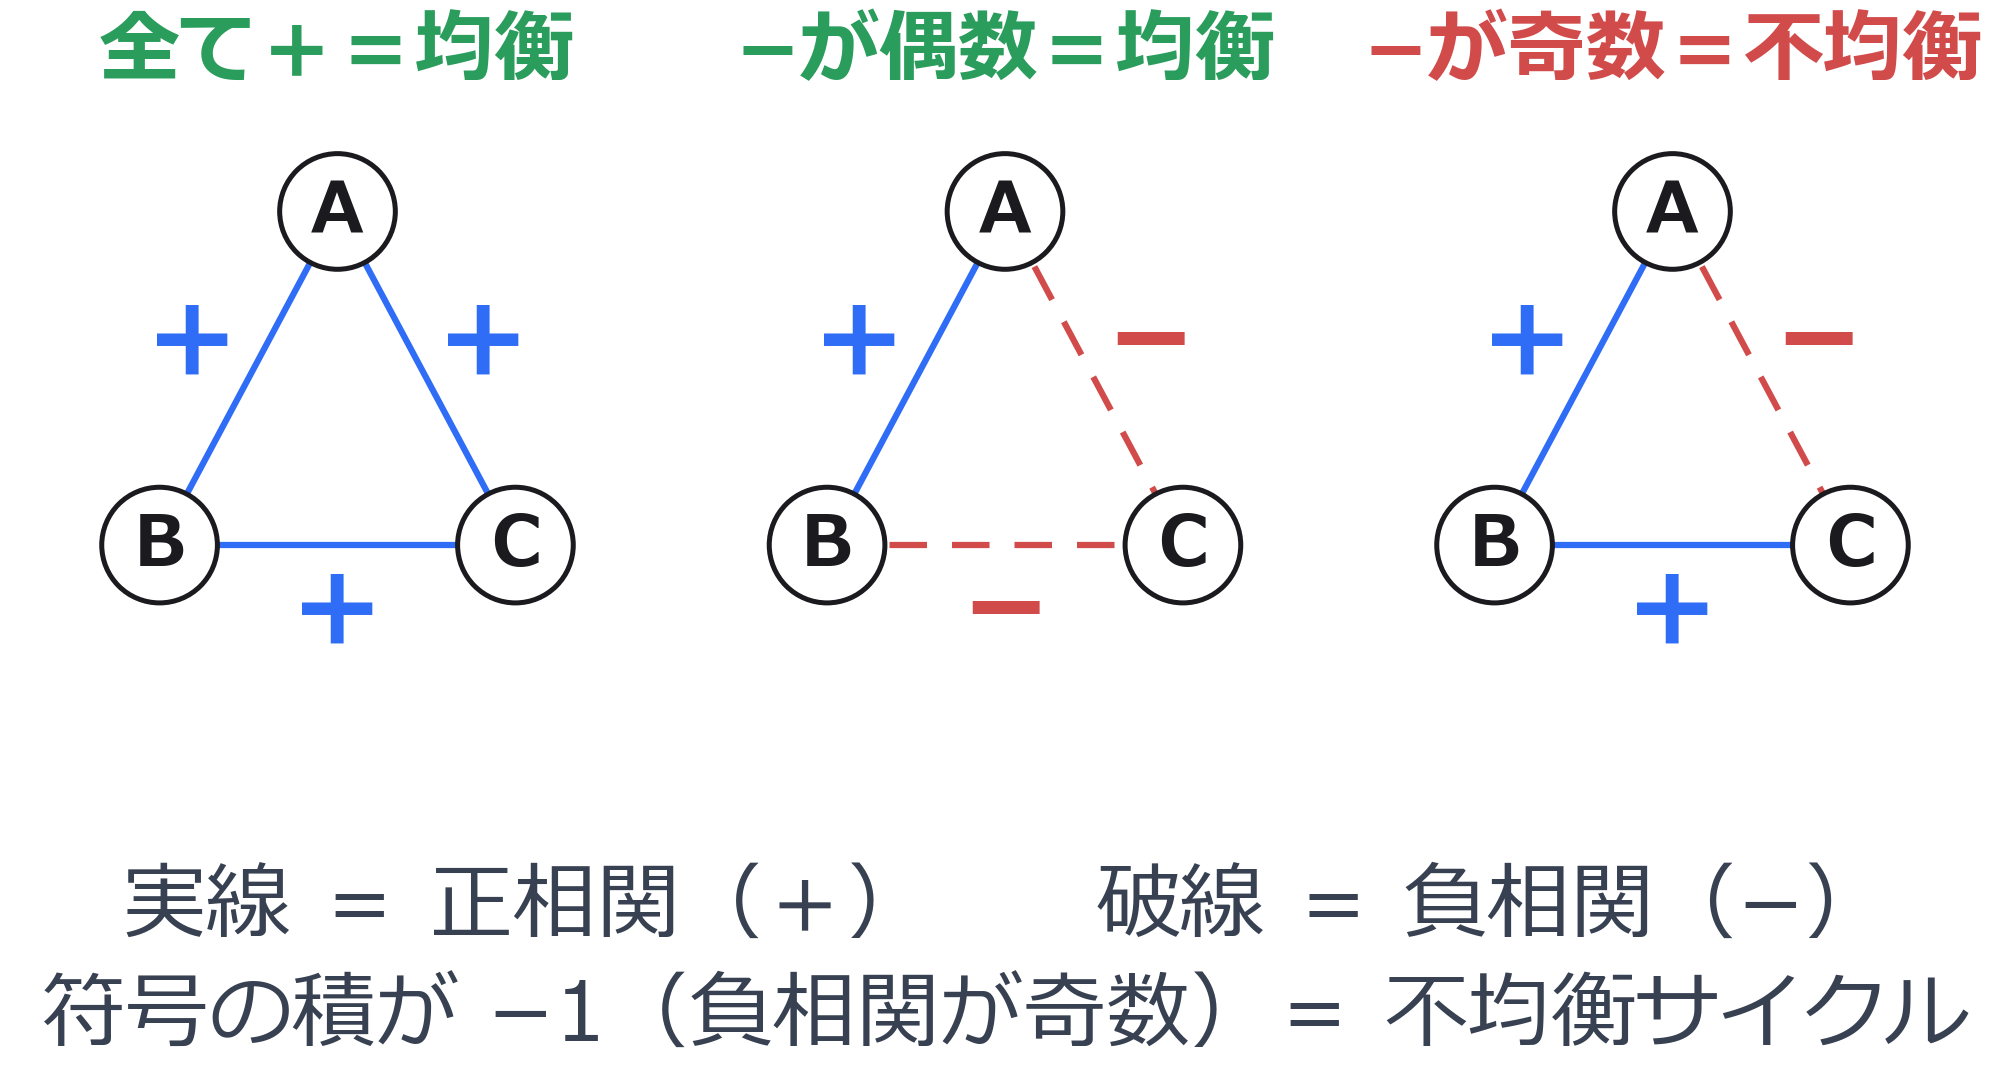
\includegraphics[width=0.9\linewidth]{../../figs/slide_balance.png}

\vspace{1mm}
\raggedright
\begin{itemize}
\setlength{\itemsep}{1mm}
\item かけ算が $+$：つじつまが合う（整合）
\item かけ算が $-$：どこかで関係がねじれている（\textbf{\color{warn}矛盾}）
\end{itemize}
指標 $\nunb$ ＝ \textbf{矛盾している輪の個数}。
}

\block{\bt{3.3}2つは独立か}{%
指標1（穴）と指標2（矛盾）は、同じネットワークから作るのに、
\textbf{たがいにどれくらい連動するか}を相関で測った。

\vspace{2mm}
\centering
\renewcommand{\arraystretch}{1.25}
\begin{tabular}{lcl}
\toprule
{\bfseries データ期間} & {\bfseries 相関} & {\bfseries }\\
\midrule
短期（5年）  & 0.15 & \color{accent}\textbf{ほぼ独立}\\
中期（10年） & 0.19 & ほぼ独立\\
中期（15年） & 0.26 & 弱い連動\\
長期（20年） & \textbf{0.40} & {\color{warn}\textbf{連動}}\\
\bottomrule
\end{tabular}

\vspace{2mm}
\raggedright
\textbf{短期と長期で対照的}:
\begin{itemize}
\setlength{\itemsep}{1mm}
\item \textbf{短期}：2指標はばらばらに動く＝\textbf{\color{accent}独立}（別々の情報）
\item \textbf{長期}：危機（2008・2020等）を多く含み、穴も矛盾も同時に跳ねて\textbf{\color{warn}連動}
\end{itemize}
}

\block{\bt{3.4}2指標の統合：$\ediv$}{%
2指標を同じ物差しに揃える\textbf{標準化 $z$}（$x_t$＝各指標のその日の値）:
\[
z(x_t) = \frac{x_t - \mathrm{mean}(x_{\le t})}{\mathrm{sd}(x_{\le t})}
\]
{\color{muted}\small mean・sd＝その日\textbf{まで}の平均・標準偏差（未来は見ない）。$z$＝過去平均から標準偏差いくつ分外れたか。}

\vspace{2mm}
2つを組み合わせた指標:
\[
\boxed{\ediv = z(\nunb) - z(L^1)}
\]
\begin{itemize}
\setlength{\itemsep}{1mm}
\item \textbf{\color{warn}$\ediv > 0$}：矛盾が穴を上回る＝\textbf{危険サイン} → 株を避ける
\item \textbf{$\ediv < 0$}：穴が矛盾を上回る＝平常 → 株を持つ
\end{itemize}
}

% ================= 右列 =================
\column{0.333}

\block{\bt{3.5}なぜ「差分」なのか}{%
片方だけでは効かない。同じ条件（危険サインの日に株を避ける）で
20年運用したときの\textbf{最大下落}:

\vspace{2mm}
\centering
\renewcommand{\arraystretch}{1.25}
\begin{tabular}{lcc}
\toprule
{\bfseries 使う指標} & {\bfseries 最大下落} & {\bfseries シャープ比}\\
\midrule
\textbf{$\ediv$（差分）} & {\color{accent}\textbf{$-20\%$}} & {\color{accent}\textbf{0.76}}\\
矛盾 $\nunb$ だけ & $-45\%$ & 0.47\\
穴 $L^1$ だけ & $-56\%$ & 0.22\\
何もしない & $-57\%$ & 0.48\\
\bottomrule
\end{tabular}

\vspace{2mm}
\raggedright
\begin{itemize}
\setlength{\itemsep}{1mm}
\item 片方だけでは\textbf{何もしないのと大差なし}
\item \textbf{\color{accent}差分にして初めて $-20\%$ に激変}
\end{itemize}
穴を基準に、矛盾の``純粋な超過''を取り出すのが差分の役割。
}

\block{\bt{4.}結果：下落を回避できた}{%
$\ediv>0$ の日に株を売って現金化する戦略を、
\textbf{シミュレーション（過去データでの模擬売買）}で検証:

\vspace{2mm}
\centering
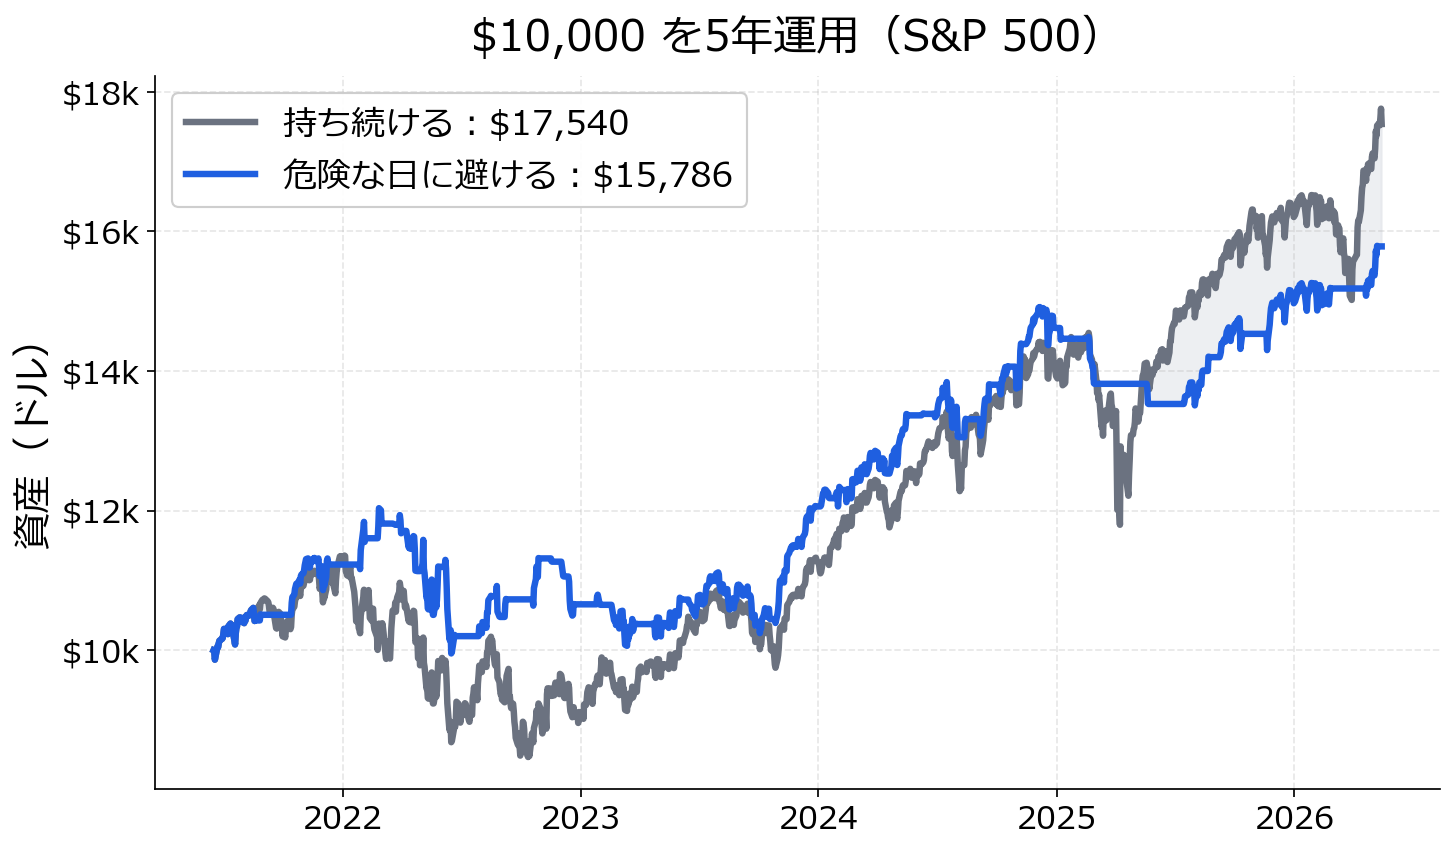
\includegraphics[width=0.9\linewidth]{../../figs/slide_equity_absolute.png}\\[1mm]
{\color{muted}\footnotesize \$10{,}000 を5年運用した模擬売買（S\&P 500、取引コスト込み）}

\vspace{1mm}
\raggedright
\begin{itemize}
\setlength{\itemsep}{1mm}
\item \textbf{最大下落が $-25\%\to-17\%$} に浅くなる
\item 20年・16回の検証でも最大下落は\textbf{ランダム回避の上位1\%}
\item ただし\textbf{リターンは持ち続けに劣る}（下落回避に特化）
\end{itemize}
}

\block{\bt{}今後の取り組み}{%
\begin{itemize}
\setlength{\itemsep}{1.5mm}
\item \textbf{他市場での再現}（欧州・アジア・暗号資産）で一般性を確かめる
\item \textbf{なぜ差分が効くのか}の理論的な解明（現状は経験的な発見）
\item 位相と符号を統一的に扱う\textbf{数理の枠組み}（コホモロジー等）
\item 暴落の\textbf{予知}への拡張（現状は初動の検知にとどまる）
\end{itemize}
}

\end{columns}

% ================= フッタ：参考文献・検証設計 =================
\block{}{%
\begin{minipage}[t]{0.48\linewidth}
\textbf{\large 参考文献}
\small
\begin{enumerate}\setlength{\itemsep}{1mm}
\item R. N. Mantegna (1999). Hierarchical structure in financial markets. \textit{Eur. Phys. J. B} \textbf{11}, 193--197.
\item M. Gidea (2017). Topology Data Analysis of Critical Transitions in Financial Networks. \textit{NetSci-X 2017}, Springer, 47--59.
\item E. Ferreira ら (2021). Loss of structural balance in stock markets. \textit{Scientific Reports} \textbf{11}.
\item D. Cartwright \& F. Harary (1956). Structural balance. \textit{Psychol. Rev.} \textbf{63}, 277--293.
\end{enumerate}
\end{minipage}
\hfill
\begin{minipage}[t]{0.30\linewidth}
\textbf{\large 検証設計}
\small
\begin{itemize}\setlength{\itemsep}{1mm}
\item \textbf{データ}: Yahoo Finance (yfinance) の40銘柄（為替・株価指数・個別株・商品・債券・暗号）、2006--2026年、日次終値
\item \textbf{前進検証}: 3年学習/1年テストを20年で16回（未来を見ない）
\item \textbf{比較}: ランダム回避1000本・VIX より最大下落が浅い
\item \textbf{因果}: 政策ショック $\to\ediv$（グレンジャー因果 $p=0.02$）
\end{itemize}
\end{minipage}
\hfill
\begin{minipage}[t]{0.18\linewidth}
\centering
\textbf{\large GitHub}\\[1mm]
{\color{muted}\footnotesize 全コード・データ公開}\\[2mm]
\qrcode[height=34mm]{https://github.com/hajimedayo328/market-graph-presentation}\\[2mm]
{\color{muted}\scriptsize 生成AI（Claude）を解析・作図・原稿に補助使用。着想・解釈は著者。}
\end{minipage}
}

\end{document}
